\chapter{Arquitectura de la solución}\label{arquitectura}

Luego de analizar las necesidades del proyecto y el estado actual de la industria frente al desafío, el siguiente paso es establecer una arquitectura base con la cual definir las partes más relevantes del sistema. En la figura \ref{arqui} se pueden apreciar las 3 secciones más importantes y detalladas más adelante. Cabe destacar que es transversal la necesidad de herramientas que permitan un rápido despliegue, con el fin de generar pruebas constantemente.

\begin{figure}[H]
	\centering
	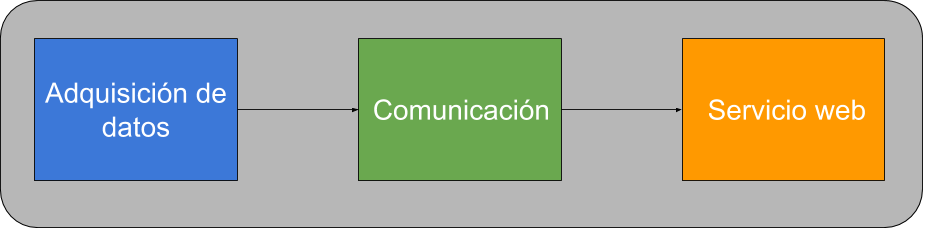
\includegraphics[scale=0.43]{figuras/arquitectura/arqui.png}
	\caption{Arquitectura referente}
	\label{arqui}
\end{figure}

\newpage
\section{Adquisición de datos}
Una primera necesidad del proyecto es la obtención y procesamiento de los datos, en una primera instancia se omitirá la definición del almacenamiento, permitiendo enfocar los esfuerzos en la selección de sensores, su interconexión y la plataforma que sustente su funcionamiento. Algunos de los requisitos en este apartado son:

\begin{enumerate}
	\item \textbf{Variedad:}
	Considerando la gama de enfermedades que se podrían cubrir, es importante contemplar una plataforma que permita trabajar con gran cantidad sensores.
	\item \textbf{Comodidad:}
	A raíz de que este apartado es el único que tendrá contacto con el paciente es importante pensar en el confort ofrecido, descartando opciones que afecten este apartado, como placas demasiado grandes o pesadas.
	\item \textbf{Flexibilidad:}
	Al estar en un proceso iterativo en búsqueda de opciones, un factor a considerar es la flexibilidad que nos puedan ofrecer las distintas opciones, permitiéndonos realizar cambios importantes sin afectar en gran medida las decisiones ya tomadas.
\end{enumerate}

\newpage
\section{Comunicación}
Dado los requerimientos del proyecto, como lo son las restricciones geográficas que impone Chile y un dispositivo de bajo costo, es necesario contemplar alternativas que no impliquen demasiada infraestructura (o que hagan uso de infraestructura ya disponible) y que además posean la penetración (o el potencial) necesaria dado el territorio nacional. Dentro de las características relevantes en este apartado, podemos encontrar:

\begin{enumerate}
	\item \textbf{Gran cobertura:}
	Considerando la envergadura inicial del proyecto, Chile, es de vital importancia que la tecnología a utilizar permita generar conexiones en la mayor parte del territorio nacional.
	\item \textbf{Alta disponibilidad:}
	Se requiere que la tecnología a emplear permita establecer conexiones a lo largo del tiempo, presentando pocas o de preferencia nulas desconexiones o incapacidades de conexión.
	\item \textbf{Escalabilidad:}
	Si bien es un aspecto dependiente de los anteriores requerimientos, es relevante considerarlo por separado como la medida que representa la capacidad de atender una gran cantidad de conexiones.
\end{enumerate}

\newpage
\section{Servicio web}
El sistema completo requiere además de los puntos anteriores, de un servicio web acorde con las necesidades del proyecto. El cual le de soporte y lo dote de mayores prestaciones, completando así un ecosistema completo en función del desafío. Entre los puntos más relevantes de este apartado se consideran:

\begin{enumerate}
	\item \textbf{Baja latencia:}
	Este proyecto se desarrolla en un marco con pacientes y posibles estados críticos de los mismos, es por ello que el tiempo de respuesta es fundamental en el servicio que se pretende ofrecer.
	\item \textbf{Alta concurrencia}
	Actualmente es común que las conexiones a servicios web tengan una alta demanda y larga duración, aumentando la concurrencia notablemente. Lo anterior es lo que se espera de un monitoreo, el cual debe ser constante en el tiempo (o al menos en una cierta ventana).
	\item \textbf{Seguridad:}
	Los datos que utilizará el sistema son totalmente privados y la protección de estos junto con los datos de conexión son un eje fundamental en la elección de tecnología a emplear, o en su defecto usar capas de seguridad anexas para brindar esta funcionalidad que se considera base.
\end{enumerate}